\documentclass[]{beamer}
%\documentclass[handout]{beamer}
%\usepackage[dvips]{color}
\usepackage{graphicx}
\usepackage{amsmath,amssymb,array,comment,eucal}
\newcommand{\e}{\mathbf{e}}
\renewcommand{\P}{\mathbf{P}}
\newcommand{\F}{\mathbf{F}}
\newcommand{\R}{\textsf{R}}
\newcommand{\mat}[1] {\mathbf{#1}}
%\newcommand{\ind}{\mathrel{\mathop{\sim}\limits^{\mathit{ind}}}}
%\newcommand{\iid}{\mathrel{\mathop{\sim}\limits^{\mathit{iid}}}}
\newcommand{\E}{\textsf{E}}
\newcommand{\SE}{\textsf{SE}}
\newcommand{\SSE}{\textsf{SSE}}
\newcommand{\RSS}{\textsf{RSS}}
\newcommand{\FSS}{\textsf{FSS}}
\renewcommand{\SS}{\textsf{SS}}
\newcommand{\MSE}{\textsf{MSE}}
\newcommand{\SSR}{\textsf{SSR}}
\newcommand{\Be}{\textsf{Beta}}
\newcommand{\St}{\textsf{St}}
%\newcommand{\C}{\textsf{C}}
\newcommand{\GDP}{\textsf{GDP}}
\newcommand{\NcSt}{\textsf{NcSt}}
\newcommand{\Bin}{\textsf{Bin}}
\newcommand{\NB}{\textsf{NegBin}}
\renewcommand{\NG}{\textsf{NG}}
\newcommand{\N}{\textsf{N}}
\newcommand{\Ber}{\textsf{Ber}}
\newcommand{\Poi}{\text{Poi}}
\newcommand{\Gam}{\textsf{Gamma}}
\newcommand{\BB}{\textsf{BB}}
\newcommand{\Gm}{\textsf{G}}
\newcommand{\Un}{\textsf{Unif}}
\newcommand{\Ex}{\textsf{Exp}}
\newcommand{\DE}{\textsf{DE}}
\newcommand{\tr}{\textsf{tr}}
\newcommand{\cF}{{\cal{F}}}
\newcommand{\cL}{{\cal{L}}}
\newcommand{\cI}{{\cal{I}}}
\newcommand{\cB}{{\cal{B}}}
\newcommand{\cP}{{\cal{P}}}
\newcommand{\bbR}{\mathbb{R}}
\newcommand{\bbN}{\mathbb{N}}
\newcommand{\pperp}{\mathrel{{\rlap{$\,\perp$}\perp\,\,}}}
\newcommand{\OFP}{(\Omega,\cF, \P)}
\newcommand{\eps}{\boldsymbol{\epsilon}}
\newcommand{\1}{\mathbf{1}_n}
\newcommand{\gap}{\vspace{8mm}}
\newcommand{\ind}{\mathrel{\mathop{\sim}\limits^{\rm ind}}}
\newcommand{\simiid}{\ensuremath{\mathrel{\mathop{\sim}\limits^{\rm
iid}}}}
\newcommand{\eqindis}{\ensuremath{\mathrel{\mathop{=}\limits^{\rm D}}}}
\newcommand{\iid}{\textit{i.i.d.}}
\newcommand{\SSZ}{S_{zz}}
\newcommand{\SZW}{S_{zw}}
\newcommand{\Var}{\textsf{Var}}
\newcommand{\corr}{\textsf{corr}}
\newcommand{\diag}{\textsf{diag}}
\newcommand{\var}{\textsf{var}}
\newcommand{\Cov}{\textsf{Cov}}
\newcommand{\Sam}{{\cal S}}
\def\H{\mathbf{H}}
\newcommand{\I}{\mathbf{I}}
\newcommand{\Y}{\mathbf{Y}}
\newcommand{\tY}{\tilde{\mathbf{Y}}}
\newcommand{\Yhat}{\hat{\mathbf{Y}}}
\newcommand{\Yobs}{\mathbf{Y}_{{\cal S}}}
\newcommand{\barYobs}{\bar{Y}_{{\cal S}}}
\newcommand{\barYmiss}{\bar{Y}_{{\cal S}^c}}
\def\bv{\mathbf{b}}
\def\X{\mathbf{X}}
\def\tX{\tilde{\mathbf{X}}}
\def\x{\mathbf{x}}
\def\xbar{\bar{\mathbf{x}}}
\def\Xbar{\bar{\mathbf{X}}}
\def\Xg{\mathbf{X}_{\boldsymbol{\gamma}}}
\def\Ybar{\bar{\Y}}
\def\ybar{\bar{y}}
\def\y{\mathbf{y}}
\def\Yf{\mathbf{Y_f}}
\def\W{\mathbf{W}}
\def\L{\mathbf{L}}
\def\w{\mathbf{w}}
\def\U{\mathbf{U}}
\def\V{\mathbf{V}}
\def\Q{\mathbf{Q}}
\def\Z{\mathbf{Z}}
\def\z{\mathbf{z}}
\def\v{\mathbf{v}}
\def\u{\mathbf{u}}

\def\zero{\mathbf{0}}
\def\one{\mathbf{1}}
\newcommand{\taub}{\boldsymbol{\tau}}
\newcommand{\betav}{\boldsymbol{\beta}}
\newcommand{\alphav}{\boldsymbol{\alpha}}
\newcommand{\A}{\mathbf{A}}
\def\a{\mathbf{a}}
\def\K{\mathbf{K}}
\newcommand{\B}{\mathbf{B}}
\def\b{\boldsymbol{\beta}}
\def\bhat{\hat{\boldsymbol{\beta}}}
\def\btilde{\tilde{\boldsymbol{\beta}}}
\def\tb{\tilde{\boldsymbol{\beta}}}
\def\bg{\boldsymbol{\beta_\gamma}}
\def\bgnot{\boldsymbol{\beta_{(-\gamma)}}}
\def\mub{\boldsymbol{\mu}}
\def\tmub{\tilde{\boldsymbol{\mu}}}
\def\muhat{\hat{\boldsymbol{\mu}}}
\def\t{\boldsymbol{\theta}}
\def\tk{\boldsymbol{\theta}_k}
\def\tj{\boldsymbol{\theta}_j}
\def\Mk{\boldsymbol{{\cal M}}_k}
\def\M{\boldsymbol{{\cal M}}}
\def\Mj{\boldsymbol{{\cal M}}_j}
\def\Mi{\boldsymbol{{\cal M}}_i}
\def\Mg{{\boldsymbol{{\cal M}_\gamma}}}
\def\Mnull{\boldsymbol{{\cal M}}_{N}}
\def\gMPM{\boldsymbol{\gamma}_{\text{MPM}}}
\def\gHPM{\boldsymbol{\gamma}_{\text{HPM}}}
\def\Mfull{\boldsymbol{{\cal M}}_{F}}
\def\tg{\boldsymbol{\theta}_{\boldsymbol{\gamma}}}
\def\g{\boldsymbol{\gamma}}
\def\eg{\boldsymbol{\eta}_{\boldsymbol{\gamma}}}
\def\G{\mathbf{G}}
\def\cM{\cal M}
\def\D{\Delta}
\def \shat{{\hat{\sigma}}^2}
\def\uv{\mathbf{u}}
\def\l {\lambda}
\def\d{\delta}
\def\Sigmab{\boldsymbol{\Sigma}}
\def\Lambdab{\boldsymbol{\Lambda}}
\def\lambdab{\boldsymbol{\lambda}}
\def\Mg{{\cal M}_\gamma}
\def\S{{\cal{S}}}
\def\qg{p_{\boldsymbol{\gamma}}}
\def\pg{p_{\boldsymbol{\gamma}}}
\def\t{\boldsymbol{\theta}}  
\def\T{\boldsymbol{\Theta}}  
\usepackage{verbatim}

\usetheme{Warsaw}
\title{Hypothesis Testing and Model Choice}
\subtitle{Merlise Clyde}
\author{STA721 Linear Models}
\institute{Duke University}
\date{\today}
\logo{duke.eps}

\begin{document}
\maketitle
\begin{frame}
  \frametitle{Estimates and t-statistics}
  \begin{itemize}
  \item MLEs do not depend on the order of the variables in the model \pause
  \item regression coefficients are adjusted for the other variables
    in the model \pause
  \item t-values correspond to test statistic for testing hypothesis
    H$_o$: $\beta_j = 0$ versus H$_a$: $\beta_j \neq 0$ given  the
    other variables are in the model \pause
  \item all p-values less than $\alpha$ does not mean that all
    coefficients are zero! \pause
 \item redundancy \pause
 \item with factors use ANOVA for simultaneous testing \pause
  \end{itemize}
\end{frame}


\begin{frame}[fragile]
  \frametitle{Estimates}
  \begin{tiny}
\begin{verbatim}
> summary(climate.lm)
Coefficients: (2 not defined because of singularities)
                               Estimate Std. Error t value Pr(>|t|)
(Intercept)                   -2.7933     2.3189  -1.205    0.235
Alkenone                       0.4463     2.3234   0.192    0.849
Faunal                         0.7235     2.4525   0.295    0.769
Sr/Ca                         -2.9254     2.5318  -1.155    0.255
Del180                        -0.3037     2.4030  -0.126    0.900
IceCore                       -3.1407     2.8504  -1.102    0.277
Pollen                        -2.6751     2.4528  -1.091    0.282
Noble Gas                     -3.2520     2.5698  -1.265    0.213
poly(latitude, 2)1            -3.0092    10.5916  -0.284    0.778
poly(latitude, 2)2            -7.3654    26.6516  -0.276    0.784
Alkenone:poly(latitude, 2)1    3.5493    10.6675   0.333    0.741
Faunal:poly(latitude, 2)1      6.5637    11.7978   0.556    0.581
Sr/Ca:poly(latitude, 2)1      11.8701    15.6097   0.760    0.451
Del180:poly(latitude, 2)1      0.8912    11.7526   0.076    0.940
IceCore:poly(latitude, 2)1         NA         NA      NA       NA
Pollen:poly(latitude, 2)1     -4.0769    13.5600  -0.301    0.765
Noble Gas:poly(latitude, 2)1  -8.7078    17.9962  -0.484    0.631
Alkenone:poly(latitude, 2)2    3.0832    26.6984   0.115    0.909
Faunal:poly(latitude, 2)2      2.8690    27.4056   0.105    0.917
Sr/Ca:poly(latitude, 2)2      19.2753    31.4567   0.613    0.543
Del180:poly(latitude, 2)2     16.1802    26.9623   0.600    0.552
IceCore:poly(latitude, 2)2         NA         NA      NA       NA
Pollen:poly(latitude, 2)2      3.3119    27.6753   0.120    0.905
Noble Gas:poly(latitude, 2)2  18.6612    30.0579   0.621    0.538

Residual standard error: 2.112 on 41 degrees of freedom
Multiple R-squared: 0.682,	Adjusted R-squared: 0.5191 
F-statistic: 4.187 on 21 and 41 DF,  p-value: 4.382e-05 

\end{verbatim}
  \end{tiny}
\end{frame}

\begin{frame}[fragile]
  \frametitle{Anova and Sequential Sum of Squares }
  \begin{small}
\begin{verbatim}
climate.lm = lm(deltaT ~ proxy *(poly(latitude,2)),
                weights=(1/sdev^2), 
                data=climate)
anova(climate.lm)
Response: deltaT
                        Df  Sum Sq Mean Sq F value    Pr(>F)    
proxy                    7 307.598  43.943  9.8541 3.848e-07 ***
poly(latitude, 2)        2  10.457   5.228  1.1725    0.3198    
proxy:poly(latitude, 2) 12  74.065   6.172  1.3841    0.2126    
Residuals               41 182.833   4.459  
\end{verbatim}
    
\end{small}

\end{frame}

\begin{frame}[fragile]
 \frametitle{Sequential Sum of Squares}
   \begin{small}
\begin{verbatim}
>anova(lm(deltaT ~ (poly(latitude,2))* proxy, weights=1/sdev^2,
          data=climate))
 Analysis of Variance Table

Response: deltaT
                        Df  Sum Sq Mean Sq F value    Pr(>F)    
poly(latitude, 2)        2  79.869  39.935  8.9553 0.0005931 ***
proxy                    7 238.185  34.026  7.6304  6.93e-06 ***
poly(latitude, 2):proxy 12  74.065   6.172  1.3841 0.2125512    
Residuals               41 182.833   4.459                      
                   
---
Signif. codes:  0 '***' 0.001 '**' 0.01 '*' 0.05 '.' 0.1 ' ' 1 
 
\end{verbatim}
\end{small}
Order Matters!
\end{frame}
\begin{frame}
  \frametitle{Decomposition}
  Consider a series of nested models: \pause
  \begin{eqnarray*}
    \M_0: \Y & = & \one_n \beta_0 + \eps   \pause\\
\M_1: \Y & = & \one_n \beta_0 + \X_1 \b_1 + \eps  \pause \\
\M_2: \Y & = & \one_n \beta_0 + \X_1 \b_1 + \X_2 \b_2 + \eps   \pause\\
\vdots & & \vdots \\
\M_k: \Y & = & \one_n \beta_0 + \X_1 \b_1 + \X_2 \b_2 + \ldots \X_k \b_k + \eps 
  \end{eqnarray*} \pause

Let $\P_j$ denote the projection on the column space in each of the
models $\M_j$: $C(\X_0, \X_1, \ldots, \X_j)$ \pause
\begin{small}
  \begin{align*}
\| \Y^T\Y \|^2 =&  \| \P_0 \Y\|^2 + \| (\P_1 - \P_0) \Y \|^2 + \|(\P_2
- \P_1)\Y\|^2 + \ldots \| (\P_k - \P_{k-1})\Y \|^2 + \\ 
& \|(\I_n -
\P_k)\Y\|^2
 \end{align*}
\end{small}

\end{frame}
\begin{frame}
  \frametitle{Sequential F tests}

  \begin{tabular}{lllc} \hline
    Hypothesis* & SS & df & F \\ \hline
$\b_1 = 0$ & $\| (\P_1 - \P_0) \Y \|^2$ & $r(\P_1) - r(\P_0)$ & $
\frac{\frac{\| (\P_1 - \P_0) \Y \|^2} {r(\P_1) - r(\P_0) }}{\shat}$
\pause \\
$\b_2 = 0$ & $\| (\P_2 - \P_1) \Y \|^2$ & $r(\P_2) - r(\P_1)$ & $ \frac{\frac{\| (\P_
2 - \P_1) \Y \|^2} {r(\P_2) - r(\P_1) }}{\shat}$  \pause \\
$\vdots$ &$\vdots$ & $\vdots$& $\vdots$ \\
 $\b_k = 0$ & $\| (\P_k - \P_{k-1}) \Y \|^2$ & $r(\P_k) - r(\P_{k-1})$ & $ \frac{\frac{\| (\P_
k - \P_{k-1}) \Y \|^2} {r(\P_k) - r(\P_{k-1}) }}{\shat}$  \pause
  \end{tabular}
  \begin{itemize}
  \item Sequential test $\b_j = 0$ includes variables from the
    previous model $\b_0, \b_1,\ldots, \b_{j-1}$ but $\b_i$ for $i >
    j$ are all set to $0$  \pause
  \item All use estimate of $\shat =  \|(\I_n -
    \P_k)\Y\|^2 /(n - r(\P_k))$ under largest model
 \pause
  \item Unless $\P_j\P_i = \zero$ for $i \neq j$, decomposition will
    depend on the order of $\X_j$ in the model  \pause
  \item If last $\X_k$ is $n\times 1$, then $t^2 = F$  for testing H$_0$:
    $\beta_k = 0$  \pause
  \end{itemize}
\end{frame}
% add here
\begin{frame}
  \frametitle{Data}
\centerline{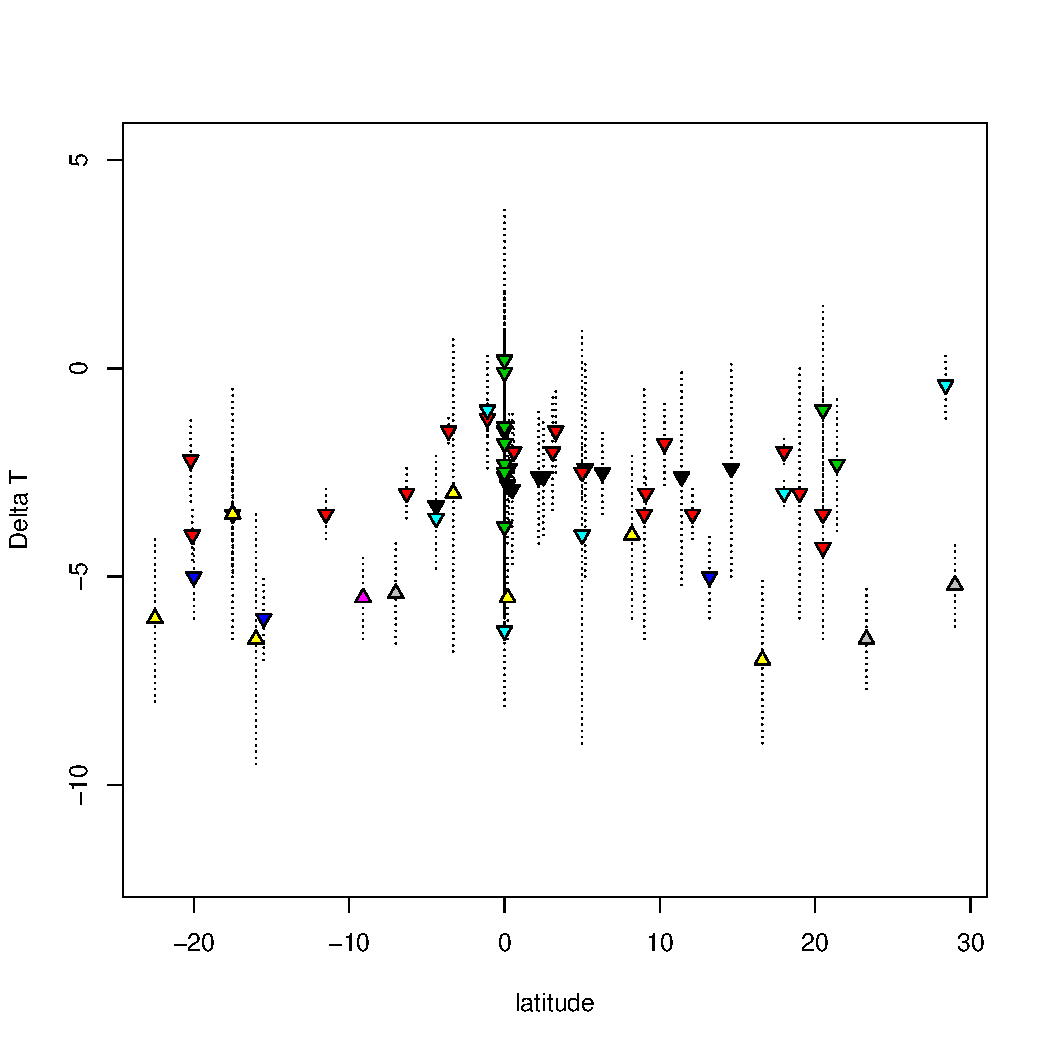
\includegraphics[height=3.5in]{temp-lat}}
\end{frame}
\begin{frame}[fragile]
  \frametitle{Order 1: Sequential Sum of Squares }
  \begin{small}
\begin{verbatim}
climate.lm = lm(deltaT ~ proxy *(poly(latitude,2)),
                weights=(1/sdev^2), 
                data=climate)
anova(climate.lm)
Response: deltaT
                        Df  Sum Sq Mean Sq F value    Pr(>F)    
proxy                    7 307.598  43.943  9.8541 3.848e-07 ***
poly(latitude, 2)        2  10.457   5.228  1.1725    0.3198    
proxy:poly(latitude, 2) 12  74.065   6.172  1.3841    0.2126    
Residuals               41 182.833   4.459  
\end{verbatim}
    
\end{small}

\end{frame}

\begin{frame}[fragile]
 \frametitle{Order 2: Sequential Sum of Squares}
   \begin{small}
\begin{verbatim}
>anova(lm(deltaT ~ (poly(latitude,2))* proxy, weights=1/sdev^2,
          data=climate))
 Analysis of Variance Table

Response: deltaT
                        Df  Sum Sq Mean Sq F value    Pr(>F)    
poly(latitude, 2)        2  79.869  39.935  8.9553 0.0005931 ***
proxy                    7 238.185  34.026  7.6304  6.93e-06 ***
poly(latitude, 2):proxy 12  74.065   6.172  1.3841 0.2125512    
Residuals               41 182.833   4.459                      
\end{verbatim}
\end{small}
\end{frame}
\begin{frame}
  \frametitle{Prediction with Latitude}
  \centerline{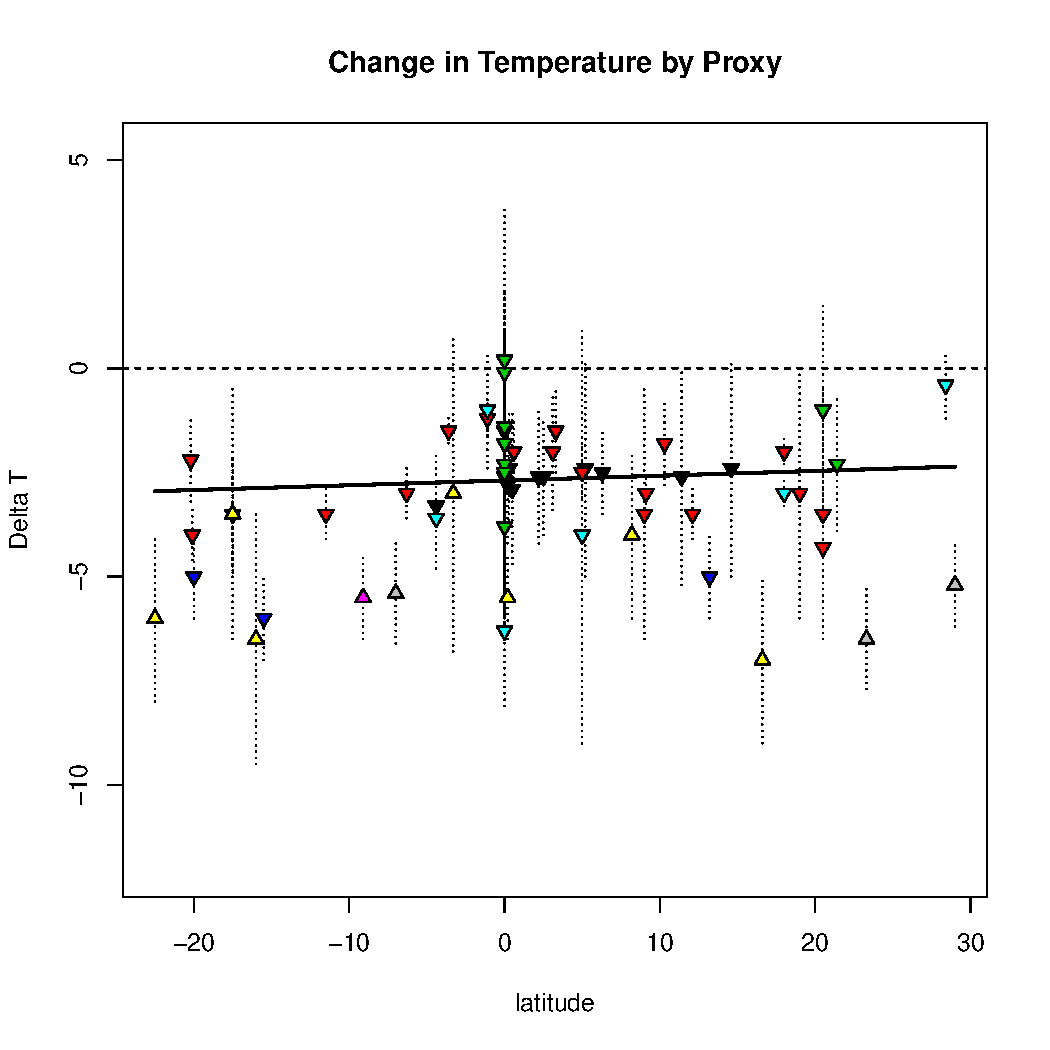
\includegraphics[height=3in]{pred-temp-lat}}
\end{frame}
\begin{frame}
  \frametitle{Added Variable Plots}
  \begin{enumerate}
  \item   Let $\P_{(-j)}$ denote the projection on the space spanned by
   $C(\X_0, \ldots, \X_{j-1}, \X_{j+1}, \ldots \X_k)$  (omit variable
    $j$) \pause
\item  Find residuals $\e_{\Y \mid \X_{(-j)}} = (\I - \P_{(-j)})\Y$
  from regressing $\Y$ on  all variables except $\X_j$ \pause
\item  Remove the effect of other explanatory variables from $\X_j$ by
  taking residuals $ \e_{\X_j \mid \X_{(-j)}} = (\I - \P_{(-j)})\X_j$ \pause
\item Plot $\e_{\Y \mid \X_{(-j)}}$ versus $\e_{\X_j \mid \X_{(-j)}}$ \pause
\item Slope is adjusted regression coefficient in full model $\mub \in
  C(\X_0, \ldots, \X_{j-1}, \X_j, \X_{j+1}, \ldots \X_k)$ \pause
\item {\tt library(car)} \pause
\item {\tt avPlots(climate1.lm, terms$=\sim .$)}
  \end{enumerate}
 \end{frame}

\begin{frame}%
   \frametitle{avPlots}
 \centerline{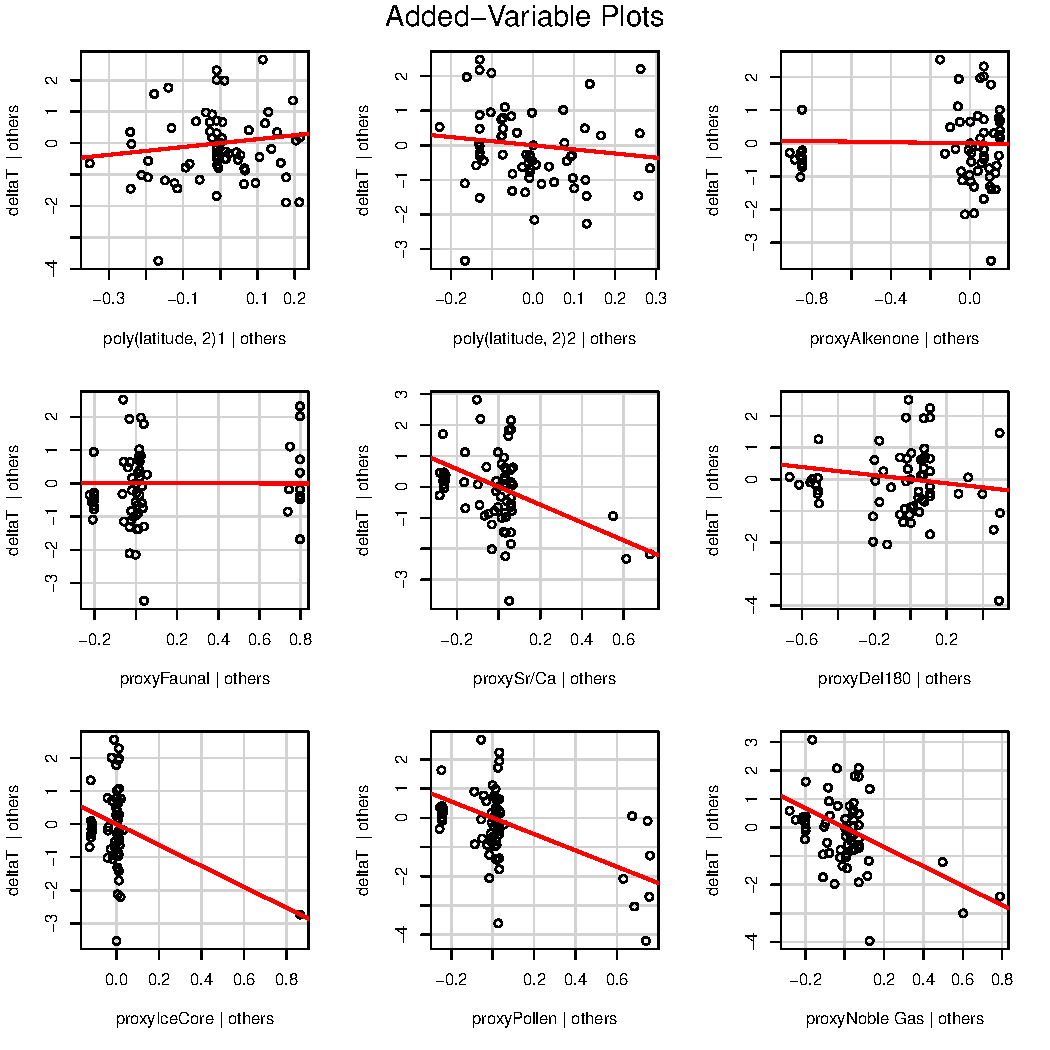
\includegraphics[height=3in]{avplot}}
 \end{frame}
\begin{frame}[fragile]
  \frametitle{Multiple Model Objects and Anova in \R}
\begin{verbatim}
> anova(climate3.lm,climate2.lm,climate1.lm, climate.lm)
Analysis of Variance Table

Model 1: deltaT ~ T.M
Model 2: deltaT ~ poly(latitude, 2) + T.M
Model 3: deltaT ~ poly(latitude, 2) + proxy
Model 4: deltaT ~ proxy * (poly(latitude, 2))
  Res.Df    RSS Df Sum of Sq      F   Pr(>F)   
1     61 385.66                                
2     59 347.11  2    38.542 4.3215 0.019814 * 
3     53 256.90  6    90.215 3.3718 0.008552 **
4     41 182.83 12    74.065 1.3841 0.212551   
---
Signif. codes:  0 '***' 0.001 '**' 0.01 '*' 0.05 '.' 0.1 ' ' 1 
\end{verbatim}
\end{frame}


\begin{frame}[fragile]
  \frametitle{Other order}
 \begin{small}
\begin{verbatim}
> anova(climate3.lm,climate2.lm,climate1.lm, climate.lm)
Analysis of Variance Table

Model 1: deltaT ~ T.M
Model 2: deltaT ~ proxy
Model 3: deltaT ~ poly(latitude, 2) + proxy
Model 4: deltaT ~ proxy * (poly(latitude, 2))
  Res.Df    RSS Df Sum of Sq      F   Pr(>F)   
1     61 385.66                                
2     55 267.35  6   118.301 4.4215 0.001555 **
3     53 256.90  2    10.457 1.1725 0.319767   
4     41 182.83 12    74.065 1.3841 0.212551   
---
Signif. codes:  0 '***' 0.001 '**' 0.01 '*' 0.05 '.' 0.1 ' ' 1 
\end{verbatim}
  \end{small}
\end{frame}
\begin{frame} \frametitle{Residual Plots}

\centerline{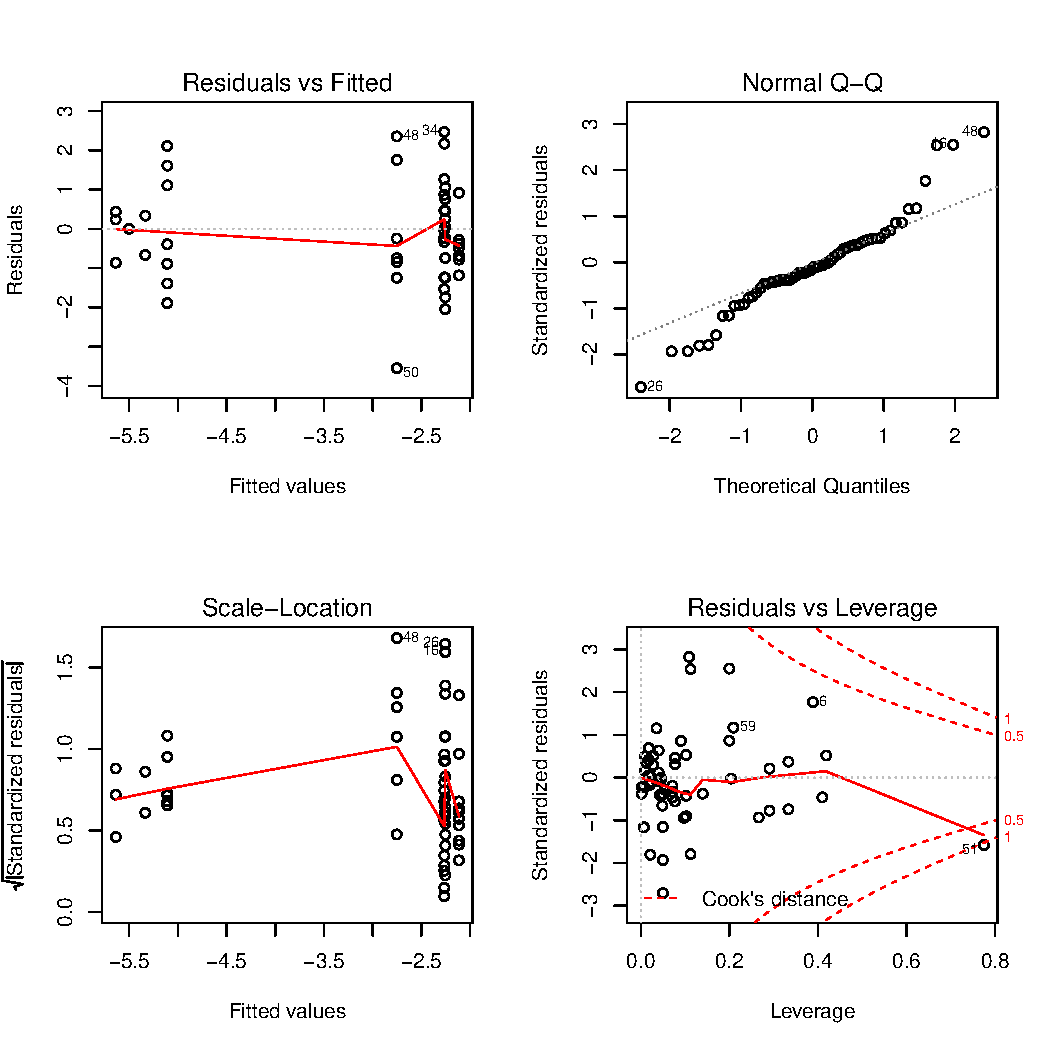
\includegraphics[height=2.5in]{resid}}
\end{frame}

\begin{frame}[fragile]
  \frametitle{Terrestrial versus Marine}
\begin{small}
\begin{verbatim}
climate.final = lm(deltaT ~ T.M + proxy -1, weights=(1/sdev^2))

               Estimate Std. Error t value Pr(>|t|)    
T.MT            -5.6360     0.7132  -7.902 1.26e-10 ***
T.MM            -2.1145     0.4124  -5.127 3.93e-06 ***
proxyAlkenone   -0.1408     0.4381  -0.321    0.749    
proxyFaunal     -0.1507     0.8971  -0.168    0.867    
proxySr/Ca      -3.2188     0.7584  -4.244 8.49e-05 ***
proxyDel180     -0.6378     0.5048  -1.263    0.212    
proxyIceCore     0.1360     1.3130   0.104    0.918    
proxyPollen      0.5283     1.0033   0.527    0.601    
proxyNoble Gas       NA         NA      NA       NA    

Multiple R-squared: 0.9115,	Adjusted R-squared: 0.8986 

          Df  Sum Sq Mean Sq  F value  Pr(>F)    
T.M        2 2635.27 1317.63 271.0625 < 2e-16 ***
proxy      6  118.30   19.72   4.0561 0.00195 ** 
Residuals 55  267.35    4.86                     
\end{verbatim}
\end{small}
\end{frame}

\begin{frame}[fragile]
  \frametitle{Even Simpler ?}
  \begin{small}
\begin{verbatim}
lm(formula = deltaT ~ T.M + I(proxy == "Sr/Ca"), weights = (1/sdev^2))

                        Estimate Std. Error t value Pr(>|t|)    
(Intercept)              -5.3915     0.4486 -12.018  < 2e-16 ***
T.MM                      3.0585     0.4649   6.579 1.30e-08 ***
I(proxy == "Sr/Ca")TRUE  -3.0003     0.6371  -4.709 1.52e-05 ***

Residual standard error: 2.166 on 60 degrees of freedom
Multiple R-squared: 0.5103,	Adjusted R-squared: 0.4939 

Model 1: deltaT ~ T.M + I(proxy == "Sr/Ca") 
Model 2: deltaT ~ T.M + proxy - 1
  Res.Df    RSS Df Sum of Sq      F Pr(>F)
1     60 281.58                           
2     55 267.36  5    14.228 0.5854  0.711
\end{verbatim}
\end{small}
\end{frame}
\begin{frame}
  \frametitle{Boxplots}
\centerline{ 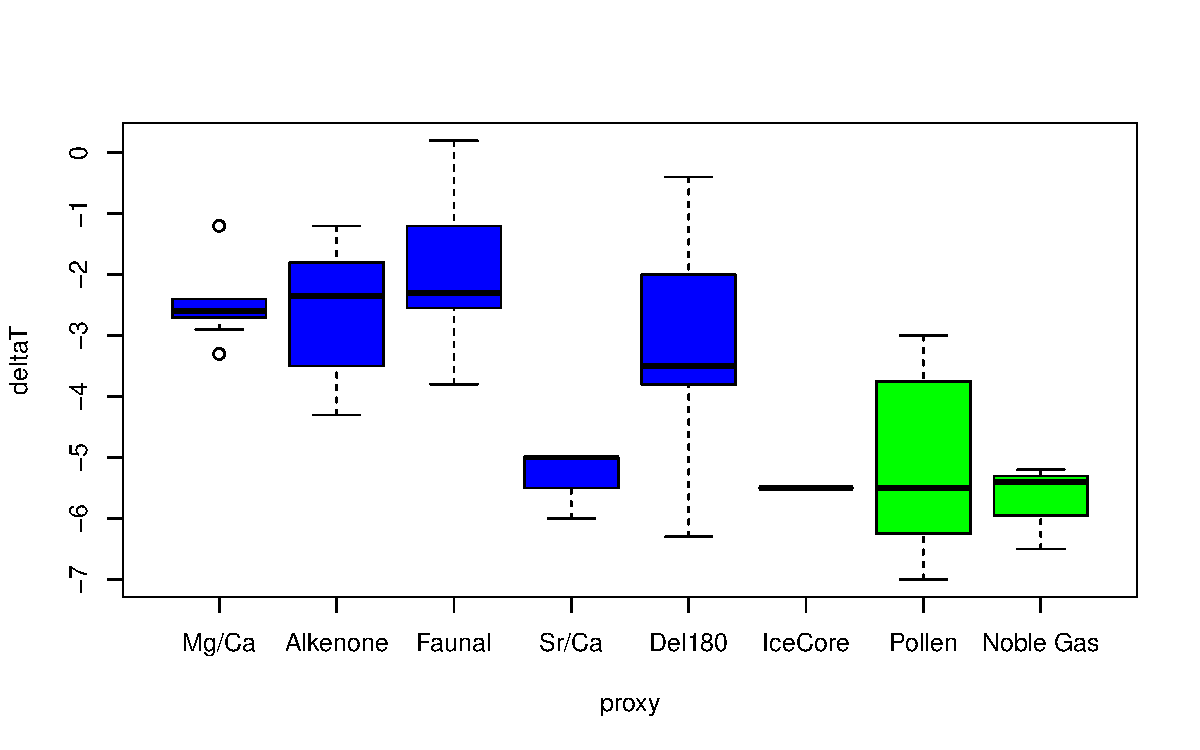
\includegraphics[height=2.5in]{box}}
\end{frame}
\begin{frame}
  \frametitle{Design}
  \centerline{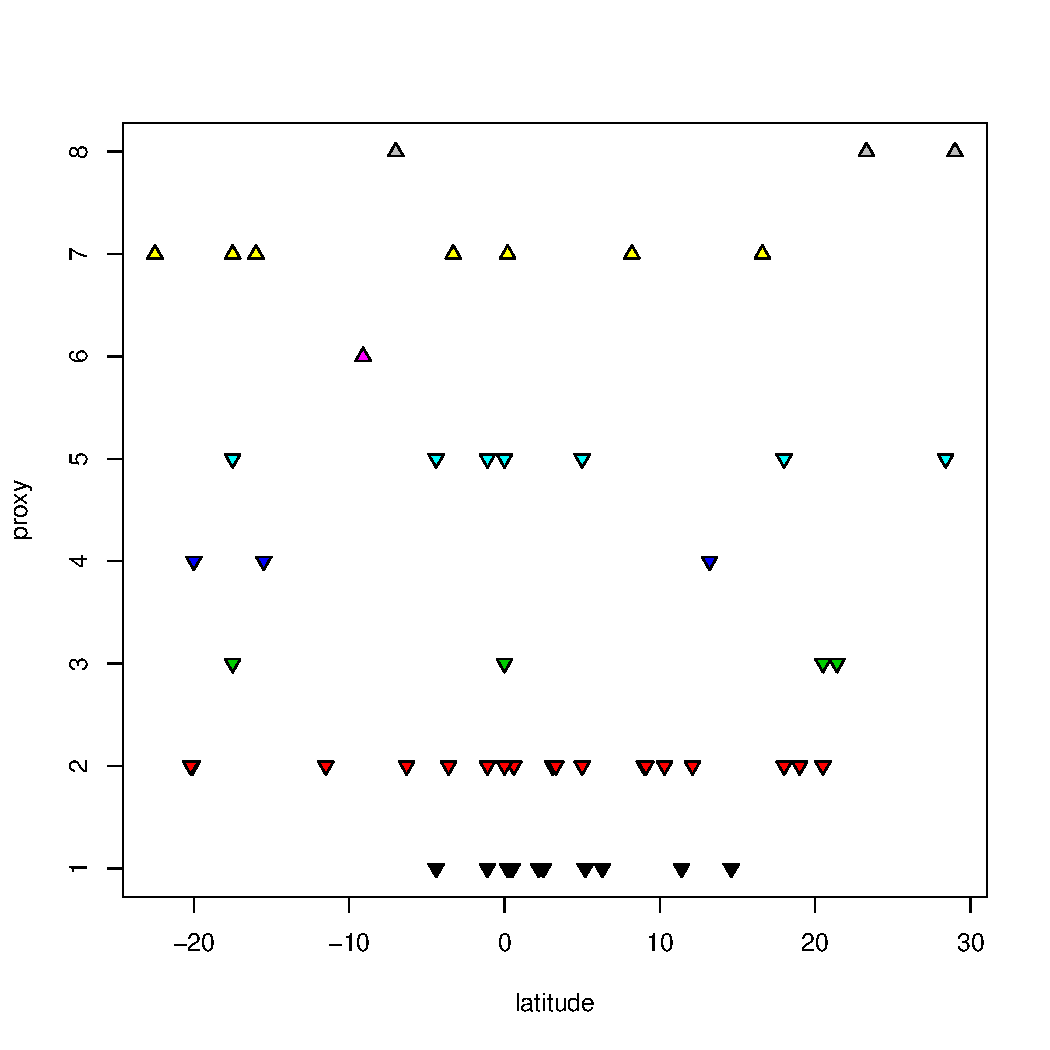
\includegraphics[height=3in]{lat-proxy}}
\end{frame}

\begin{frame}
  \frametitle{Summary}
  \begin{itemize}
   \item Ignoring proxies, there are systematic trends with
     latitude. \pause
  \item Difference among proxies, even after adjusting for latitude \pause
\item Weak evidence of a latitude effect, after taking into account proxies
\pause
 \item  Terrestrial sites differ from Marine sites, however there are significant difference among
      proxies within the Marine group  driven by the {\tt Sr/Ca} proxy which
      indicates a significantly greater increases in temperatures 
\pause
   \item Significant warming for Terrestrial ($5.4 ^\circ C$) with
     Marine  sites   significantly  cooler ($3^ \circ  C$)\pause 
   \item {\tt Sr/Ca} proxies are significantly cooler than other
     marine proxies by about $3^\circ C$ \pause
  \end{itemize}

Uncertainty Measures?  \pause  Normal Assumptions? 
\end{frame}

\end{document}
